\newpage
\subsection{Messung der Linearität beim Ausschlagverfahren}\label{sec:1-4}
\subsubsection{Aufgabenstellung}

Hier soll der nichtlineare Ausschlag am Anzeigeinstrument (AI) bei großen Widerstandsänderungen beobachtet werden. Hierzu werden zunächst die Brückenwiderstände $R_2$, $R_3$ und $R_4$ auf $\SI{1}{\kilo\ohm}$ eingestellt und die Brücke anschließend am Steckplatz $R_1$ mit einer Widerstandsdekate Abgeglichen. Für die Messung wird $R_2'=R_2 + \Delta R$ auf alle Werte zwischen \SI{100}{\ohm} und \SI{10}{\kilo\ohm} durchgeschalten. Anschließend wird die Auschlagspannung $U_0$ gemessen und mit der Berechnung von $U_0 = f(\Delta R)$ verglichen.

\subsubsection{Verwendetes Material}

\begin{table}[h]
	\centering
	\caption{Verwendetes Material}
	\begin{tabularx}{\textwidth}{XXX}
		\textbf{Material} & \textbf{Verwendung} & \textbf{Anmerkungen}\\ \midrule
		HM8001 & Hilfsspannung ($U_H$) & $U_H=\SI{3}{\volt}$ \\
		M-4600 & Ausschlaginstrument ($U_0$) & Bezeichung: AI \\
		RS-200 & Abgleichwiderstand ($R_1$) & $\pm (\SI{1}{\percent} + \SI{0.025}{\ohm})$\\
	\end{tabularx}	
\end{table}

\subsubsection{Versuchsaufbau}

Das Labornetzteil wurde auf $U_H=\SI{3}{\volt}$ eingestellt. Beim Abgleichen der Brücke ergab sich ein Widerstand von $R_1=\SI{1002}{\ohm}$. Da dieser Wert sehr nahe an \SI{1}{\kilo\ohm} liegt, wird in den rechnungen $R_1 = R_2 = R_3 = R_4 = R$ gesetzt. 

\begin{figure}[h]
	\centering
	\begin{circuitikz}[scale=0.9, transform shape]
		\draw (0,4) to[open, v=$U_H$, o-o] (0,0)
			-- ++(2, 0) coordinate (k1)
			to[R=$R + \Delta R$, *-] ++(0,2) coordinate (k2)
			to[vR=$R$, -*] ++(0,2) coordinate (k3)
			-- ++(-2,0);
		\draw (k1) -- ++(3,0)
			to[R=$R$] ++(0,2) coordinate (k4)
			to[R=$R$] ++(0,2) -- ++(-3,0);
		\draw (k2) to[ai, v^=$U_0$, *-*] (k4);
		\node[yshift=-20pt] at ($(k2)!0.5!(k4)$) {$R_0$};
	\end{circuitikz}
	\caption{Schaltung}
\end{figure}

\subsubsection{Berechnungen}

Zur Berechnung von $U_0 = f(R_2')$ wird \cite[S.~41, Gl.~2.3]{EMTPraktikum2025} herangezogen. Da das Messgerät wieder einen hinreichend großen Innenwiderstand aufweist, kann der Term im Nenner vernachnlässigt werden.
\[
U_0 = U_H\frac{R_2' R_3 - R_1 R_4}{(R_1 + R_2')(R_3 + R_4)+ \frac{1}{R_0}(\cdots)}
\]
Mit der Substitution $R_2' = R_2 + \Delta R$ und $R_1 = R_2 = R_3 = R_4 = R$, vereinfacht sich die Gleichung:
\begin{equation}
U_0(\Delta R) = U_H\frac{(R + \Delta R) R - R^2}{(2R + \Delta R)2R} = \frac{U_H}{2}\frac{\Delta R}{2R + \Delta R}\label{eq:u0}
\end{equation}
Um nun die Tangente im Abgleichfall zu bestimmen, bildet man die Ableitung an der Stelle $\Delta R = \SI{0}{\ohm}$:
\[
\frac{dU_0}{d\Delta R}\Bigg{|}_{\Delta R = 0} = \frac{U_H}{2} \left(\frac{1}{2 R + \Delta R} - \frac{\Delta R}{\left(2 R + \Delta R\right)^{2}}\right) \Bigg{|}_{\Delta R = 0} = \frac{U_H}{4R} = \SI{750}{\micro\volt\per\ohm}
\]
Die Geradengleichung für die Tangente als Funktion von $R_2'$ mit $\Delta R = R_2' - \SI{1000}{\ohm}$ ist somit:
\[
g(R_2') = \SI{750}{\micro\volt\per\ohm}\cdot(R_2'-\SI{1000}{\ohm})
\]

\subsubsection{Messergebnisse}

Die mit \autoref{eq:u0} Berechneten und gemessenen Werte sind in \autoref{tab:nonlin} dargestellt.

\begin{table}[h]
	\centering
	\caption{Messergebnisse der Ausschlagspannung}\label{tab:nonlin}
	\begin{tabularx}{\textwidth}{YYYY}
		$R_2'$ / \si{\ohm} & $\Delta R$ / \si{\ohm} & $U_{0,\text{meas}}$ / \si{\volt} & $U_0 = f(R_2)$ / \si{\volt}\\ \midrule
		$100$   & $-900$ & $-1.200$ & $-1.227$ \\
		$220$   & $-780$ & $-0.937$ & $-0.959$ \\
		$470$   & $-530$ & $-0.529$ & $-0.541$ \\
		$1000$  & $0$    & $0.000$ & $0.000$ \\
		$2200$  & $1200$ & $0.552$ & $0.562$ \\
		$4700$  & $3700$ & $0.956$ & $0.974$ \\
		$10000$ & $9000$ & $1.207$ & $1.227$ \\
	\end{tabularx}
\end{table}

\begin{wrapfigure}[12]{r}{.5\textwidth}
	\centering
	\vspace{-16pt}
	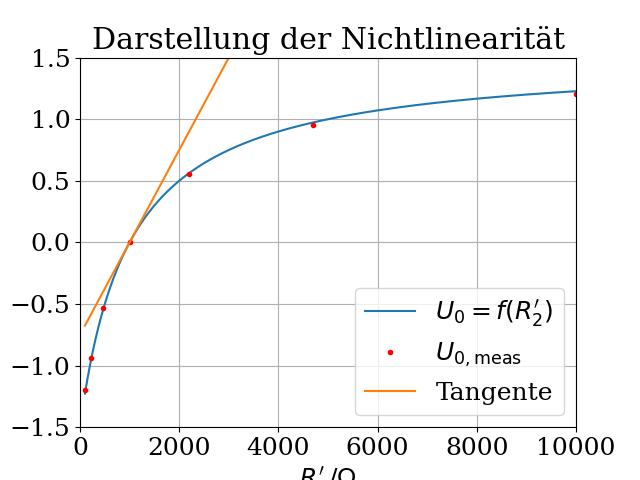
\includegraphics[width=.5\textwidth]{images/nonLin.png}
	\caption{Darstellung der Nichtlinearität für große Widerstandsänderungen}\label{fig:nonlin}
\end{wrapfigure}

Ein Plot zeigt das nichtlineare Verhalten der Funktion $U_0(R_2')$ mit $R_2' =
\Delta R - \SI{1000}{\ohm}$. Weiters ist hier auch die Tangente eingezeichnet,
mit welcher der Ausschlag nahe dem Abgleichpunkt linear angenähert werden kann.

\subsubsection{Erkenntnisse}

Man stellt fest, dass die Tangente der Empfindlichkeit der Abgleichbrücke
entspricht. Man kann erkennen dass die Messpunkte in \autoref{fig:nonlin} sehr
nahe am theoretischen Funktionsgraphen liegen, wodurch die Messergebnisse
bersttigt werden. 

